\begin{document}
\sectiontitle{6}{Functional Electrical Stimulation Setup}
\setstretch{1.6}
Before moving on to open and closed loop FES implementations it was necessary to determine the parameters of the stimulation waveform itself, as well as validate the functionality of the hardware and software implementations to ensure accurate alignment of input and output. The parameters established here form the basis for all subsequent FES stimulation in this project.

\subsection{Methods}
To determine the parameters of the setup of the FES, papers (\cite{peckham_functional_2005}, \cite{lynch_functional_2008}, \cite{marquez-chin_functional_2020}, \cite{bigland-ritchie_muscle_2000}) and a book \cite{wood_chapter_2020} on FES were consulted  . The objective was to gain a solid understanding of the impact of each parameter. Based on those insight and a comparison with typical FES implenetation, specifically for gait (e.g. \cite{aout_effects_2023} and the sources therein), appropriate parameters were selected. 

Thereafter, some changes were made to the code in order to align expected input with output. The final system was then tested by applying different stimulation parameters to every hardware channel. The channels were connected to a 1k\ohm resistance allowing for the observation of output on an oscilloscope. 
\todo{oscilloscope fig}

\subsection{Stimulation Design}
\todo{description}
\subsubsection{Waveform}
Stimulus waveforms are generally monophasic or biphasic as seen in figure \ref{fig:twowave}. Monophasic waveforms consist of a single phase of electrical current delivered in one polarity, while Biphasic waveforms consist of a cathodic phase followed by an anodic phase. This mitigates the buildup of charge at the electrode-tissue interface by ensuring that the net charge delivered over time is zero, effectively reducing the risk of tissue damage as compared to monophasic waveforms \cite{peckham_functional_2005}. The biphasic rectangular stimulation is the most commonly used, as it offers the best force-amplitude ratio \cite{lynch_functional_2008}. The balanced biphasic rectangular waveform was therefore chosen for the stimulation protocol used in this project.
 \begin{figure} [H]
     \centering
     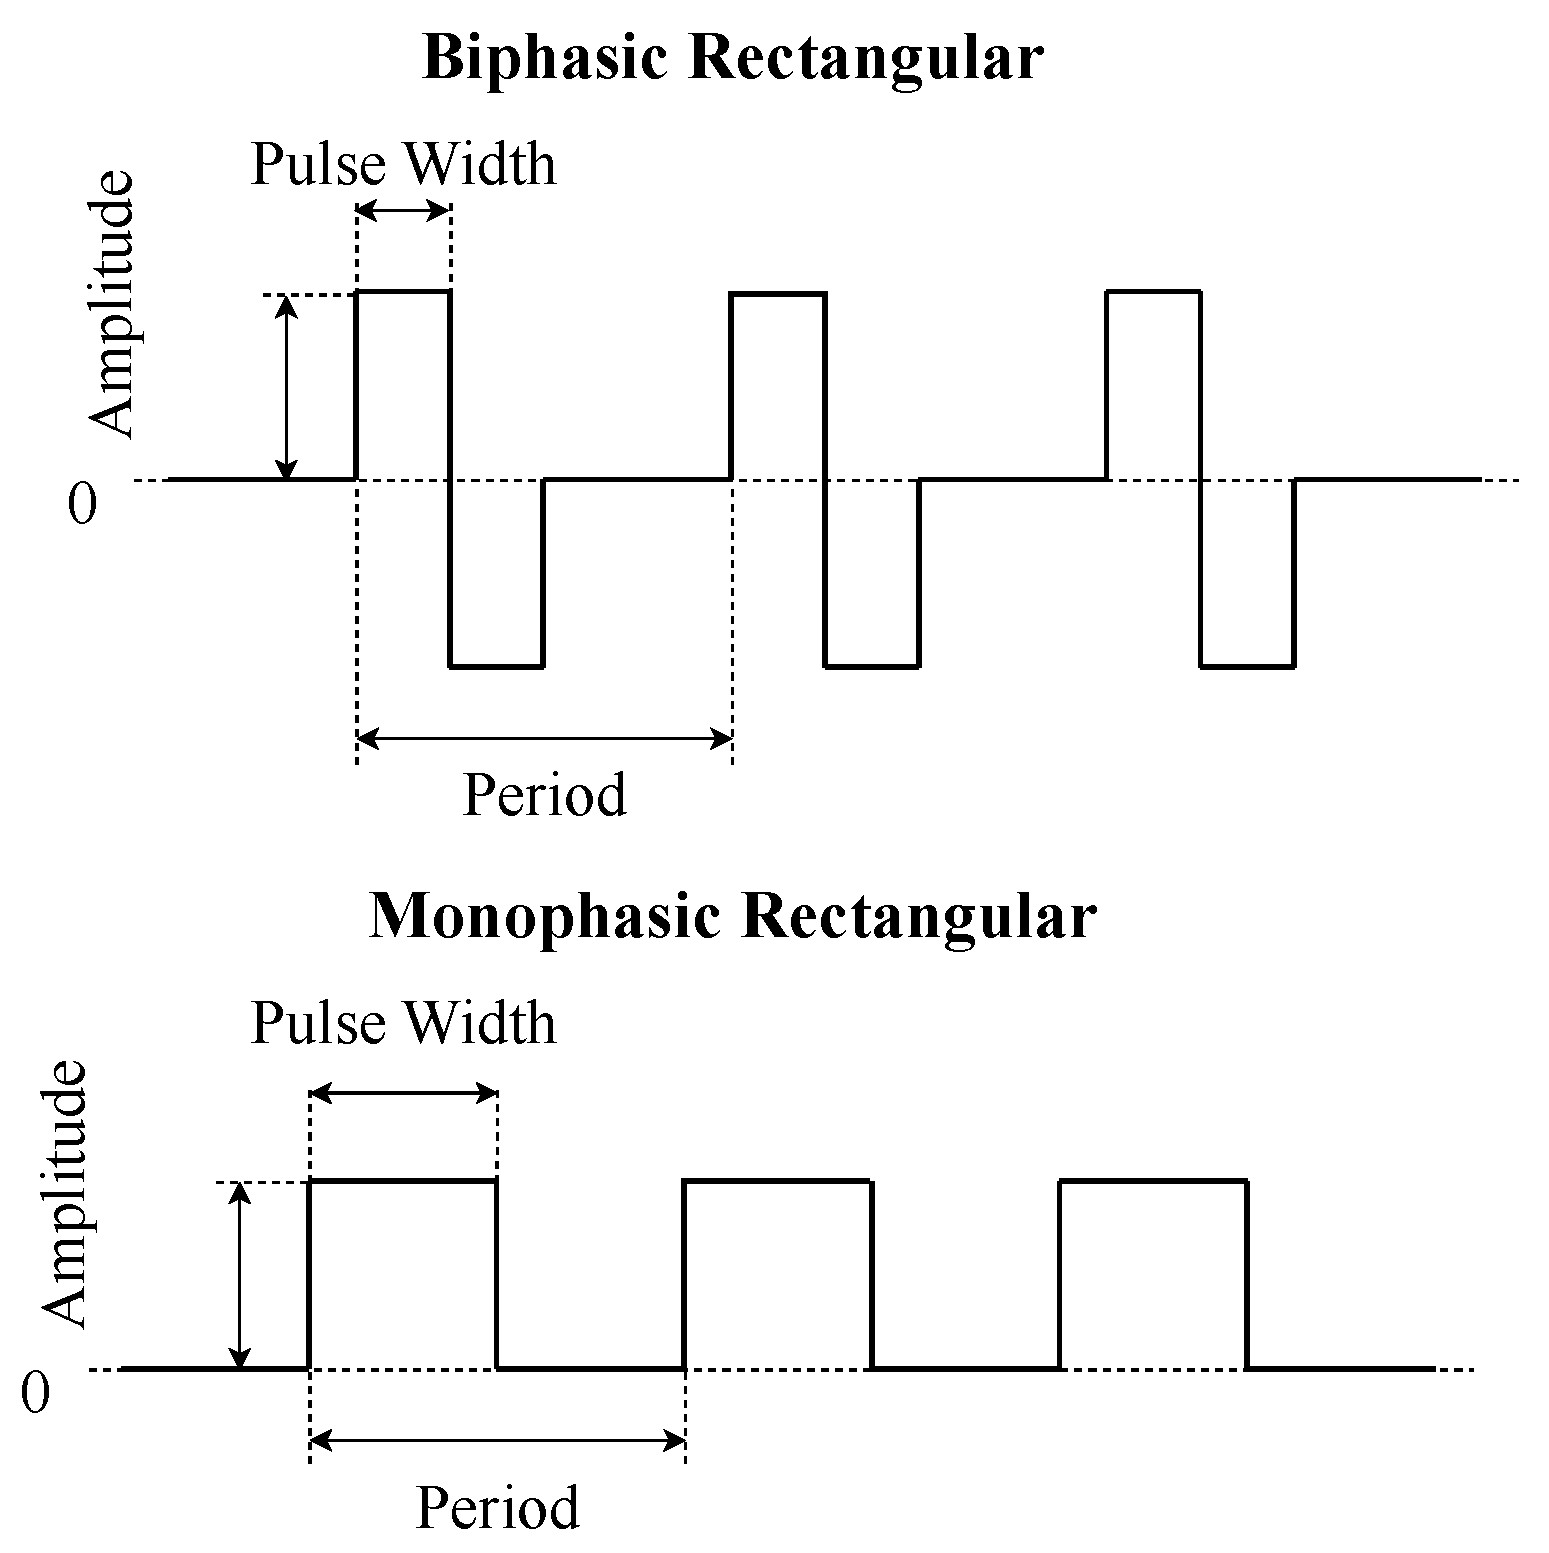
\includegraphics[width=0.6\linewidth]{images/twowaveform.jpg}
     \caption{Monophasic and Biphasic stimulation waveforms}
     \label{fig:twowave}
 \end{figure}

 \subsubsection{Frequency}
 The stimulation frequency affects the strength of the contraction and its quality. A higher frequency will lead the force produced by each subsequent pulse to be added such that the mean force of the contraction is greater than that produced by a single twitch. Further increase in frequency results in sustained contraction which produces a smooth movement instead of individual twitches. The minimum frequency required to induce fairly consistent contraction is between 16 and 20 Hz \cite{marquez-chin_functional_2020}. A smoother contraction is also more comfortable for the patient \cite{wood_chapter_2020}. However one should not use a higher frequency than necessary since fatigue accumulated in a muscle is related to the number of pulses received \cite{bigland-ritchie_muscle_2000}. Readers unfamiliar with muscle fatigue are referred to \cite{thrasher_reducing_2005}.

\begin{figure} [H]
    \centering
    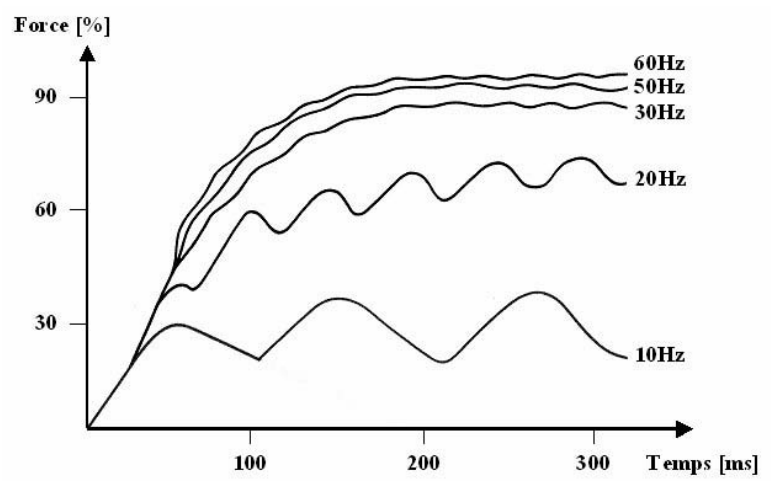
\includegraphics[width=0.7\linewidth]{images/stimfreq.png}
    \caption{Effect of stimulation frequency on force generation \cite{metrailler_systeme_2005}}
    \label{fig:stimfreq}
\end{figure}

When choosing the stimulation frequency the aim was therefore to choose the lowest frequency that produced sustained contractions. In a clinical environment, the typical range of frequencies is around 20-50Hz \cite{rupp_functional_2021}, and during literature review it was noted that the majority of teams using FES on gait are using a stimulation frequency around 40Hz \cite{aout_effects_2023}. Therefore the same 40Hz stimulation frequency was chosen for this project.

\subsubsection{Intensity}
The stimulation intensity is determined by the pulse duration as well as the pulse amplitude. To vary the intensity one of the parameters is therefore often kept constant while the other is tuned. 

 \todo{explain better why modulating w amplitude?} 
The pulse duration (pulse width) is the timespan of the stimulation pulse. Higher pulse widths result in more pronounced contraction and enable deeper tissue penetration of the stimulation. Most studies attempting FES for gait employ pulse widths spanning from 200 to 400 \micro s \todo{source}. The majority keep the pulse duration fixed at 300 \micro s and only vary the amplitude in order to set the stimulation intensity.\cite{aout_effects_2023}

The amplitude of the stimulation determines which muscles are contracted and the strength of the contraction \cite{marquez-chin_functional_2020}. Larger amplitudes recruit a larger proportion of the muscle fibers, including those located deeper. 

\begin{figure} [h]
    \centering
    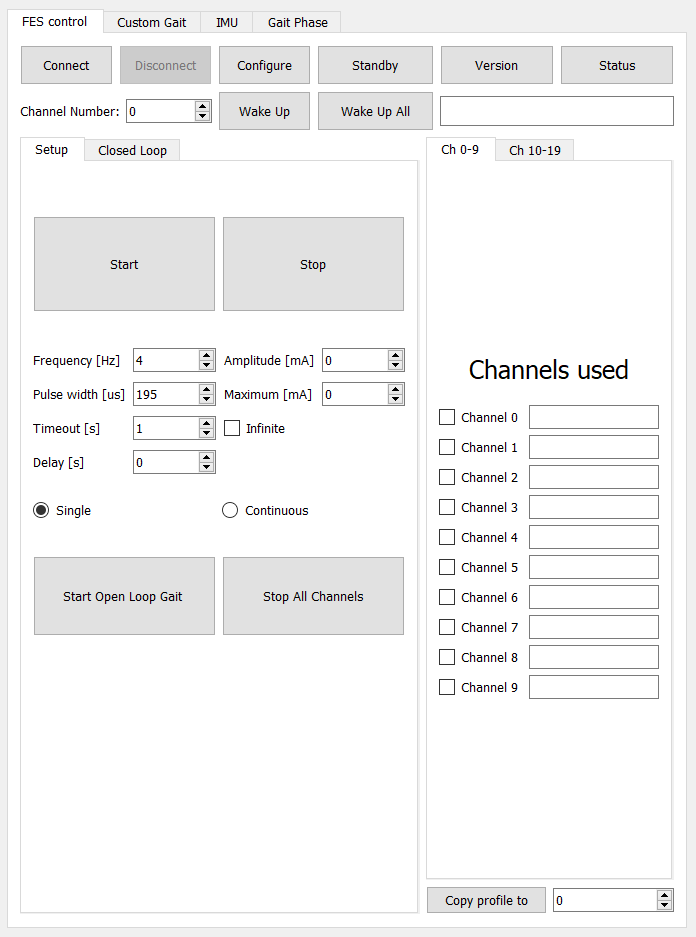
\includegraphics[width=0.65\linewidth]{images/setupgui.png}
    \caption{Graphical User Interface for setting up and finding stimulation thresholds}
    \label{fig:setupgui}
\end{figure}

Several clinically important values for the amplitude can be identified. The first is the motor threshold, which is the minimum intensity resulting in a visible muscle contraction, but not necessarily a movement \cite{marquez-chin_functional_2020}. The second is the Maximum tolerable intensity, which is the maximum amplitude that the person can sustain without pain \cite{marquez-ching_funcitonal_2020}. Finally there is the operational stimulation amplitude, the amplitude that produces the intended functional movement needed for the gait cycle. 

These thresholds are highly variable and dependent on both muscle and subject. In this project they are therefore determined experimentally by slowly ramping up the amplitude for one muscle at a time using the graphical interface in figure \ref{fig:setupgui}. Noting when a motor and thereafter, maximum tolerable intensity thresholds are reached. Based on these values and feedback from the patient an operational stimulation amplitude is set somewhere between these thresholds. 

\subsubsection{Electrode configuration}
There are two main configuration for electrical activation of neuromuscular tissue. There is bipolar stimulation in which each stimulation cite has an active electrode placed near the peripheral nerve and a reference electrode close by. The other configuration is monopolar, where the return electrode is placed in a remote area near less excitable tissue \cite{peckham_functional_2005}. 
This approach reduces the number of leads and electrodes required. However, for multichannel systems bipolar stimulation may allow greater selectivity of activation since each electrode pair creates a more localized electric field \cite{grandjean_recruitment_1986}. This, and the fact that compatible cables were available since this configuration was used in a similar project were the main reasons as to why bipolar stimulation was chosen for this project.

\subsection{Implementation}
\subsubsection{Hardware}
The hardware used for the functional electrical stimulation was the StimWave developed at the REHassist lab. It consists of 10 channels where each channel is controlled via an RS-232 line in a master/slave manner. Each electrostimulation channel (slave) has its own address and every command from the FES Gait Control software (master), is dedicated to only one channel. Such that each channel can be used to apply FES to one muscle stimulation site. There is a protocol that describes what each 3 byte command encodes. Using this encoding, the pulse frequency, pulse width, and current amplitude may be adjusted. Along with other commands such as start, stop and status commands. 

\begin{figure} [h]
    \centering
    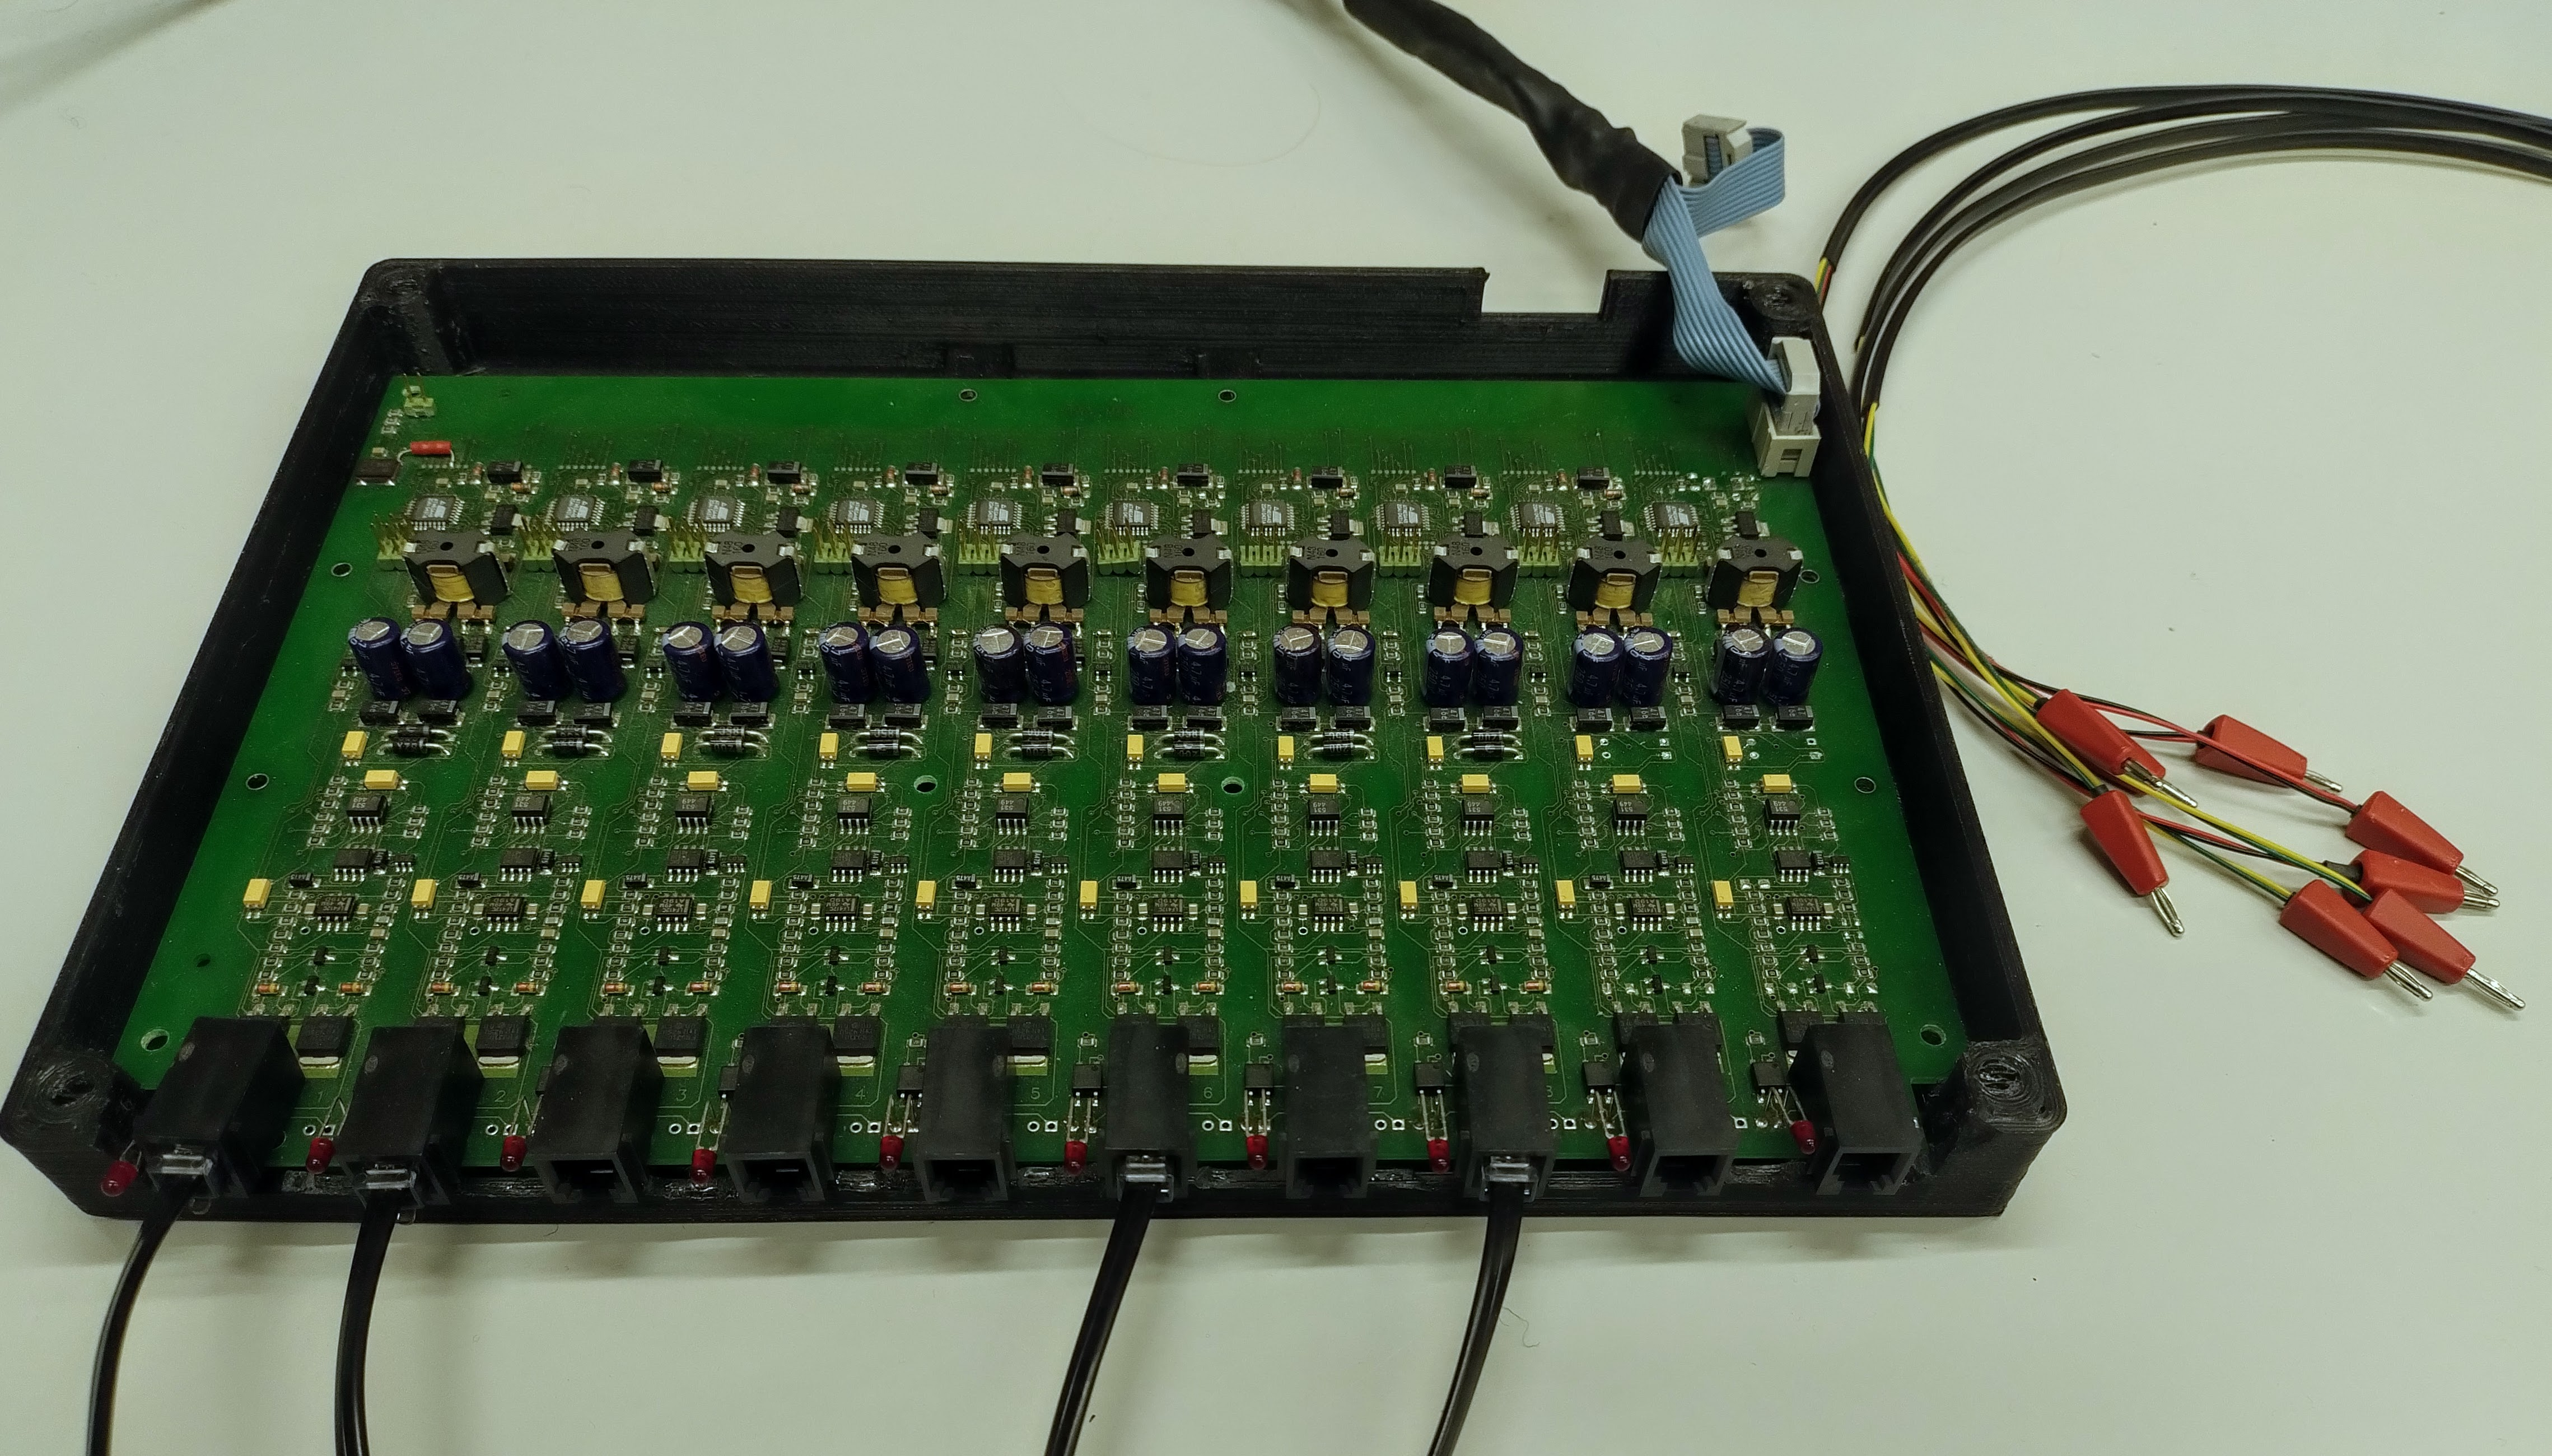
\includegraphics[width=0.8\linewidth]{images/stimwave.jpg}
    \caption{StimWave hardware utilized for FES}
    \label{fig:stimwave}
\end{figure}

In order to realize the bipolar electrode configuration cables with two banana connectors, visible in figure \ref{fig:stimwave} were used. 

\subsubsection{Software}
In terms of software there was already viable code in the code base that allowed for the setting of stimulation parameters via the GUI displayed in figure \ref{fig:setupgui}. However, the protocol for setting pulse width and frequency had been changed since the implementation used in the original code base. The translation of pulsewidth and frequency in the code therefore needed to be adjusted to the correct 7 bit selection code thereby creating the correct 3 byte commands in the new \texttt{MessageHandler} class.

\subsection{Results}
The results of the final testing of the FES system showed that the changes in software lead to the correct frequency, pulse width and amplitude outputs corresponding to outputs. However it also showed that channel 9 and 10 were not working as expected, failing to respond to any commands. After discussion with previous users it was made clear that this was however, a hardware issue that had persisted before the start of this project. Thankfully those channels would not be necessary for the implementation of the open or closed loop systems. The overall result of the setup was therefore deemed successful.

\subsection{Discussion}
The choice of stimulation parameters is an important step towards achieving effective stimulation while minimizing discomfort and muscle fatigue. This literature based approach to choosing the parameters aims to rely on the wide body of knowledge already available and ensure that the parameters adhere to clinical standards. The choice of adapting the current amplitude by experimentally determining thresholds for each subject also ensures patient-specific adaptability. The results showed that the setup should provide a robust foundation for both the open and closed-loop FES applications.

\end{document}